\begin{frame}
  \frametitle{Perché fisica e plankton?}

  \includegraphics[width=\textwidth]{../img/pribilof_oli_2014265_lrg}
  {\tiny (https://earthobservatory.nasa.gov/images/85043/coloring-the-sea-around-the-pribilof-islands)}
  {\tiny (\textit{Artificial mixing to control cyanobacterial blooms: a review}, Visser, Huisman et al.}

\end{frame}

\begin{frame}
  \frametitle{Perché fisica e plankton?}
  \begin{columns}

    \column{.5\textwidth}
    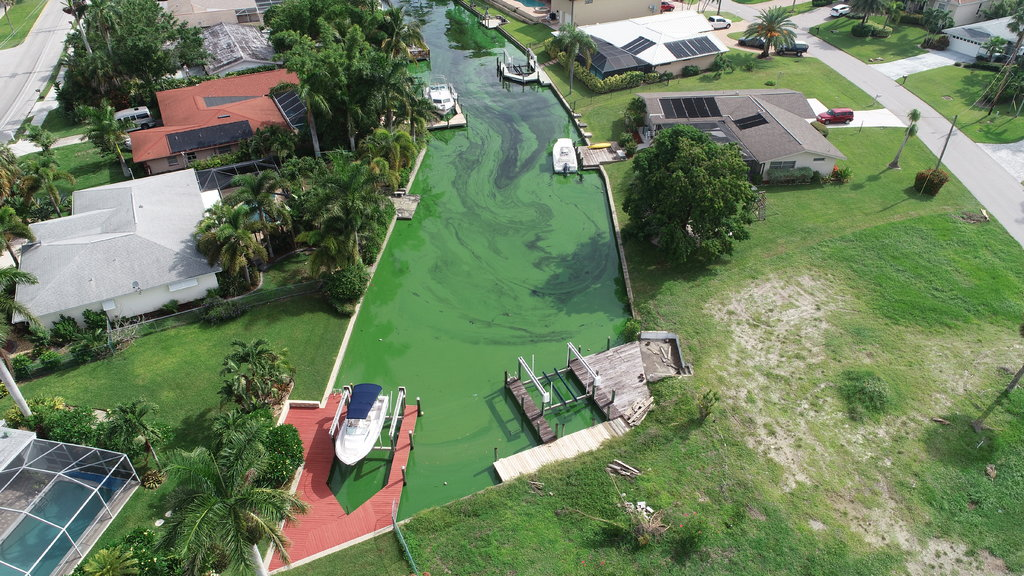
\includegraphics[width=\textwidth]{../img/toxic_bloom_florida}
    \\
    {\tiny (https://www.nytimes.com/2018/07/09/us/algae-blooms-florida-nyt.html)}
    \column{.5\textwidth}
    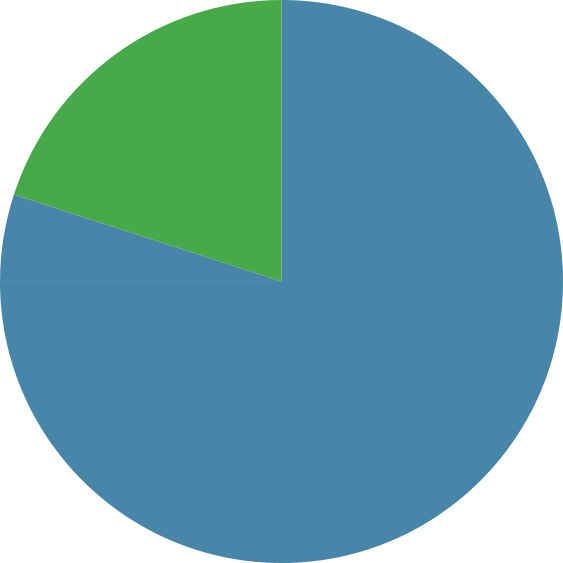
\includegraphics[width=\textwidth]{../img/70percO2}
    \\
    {\tiny Sekerci, Y. and Petrovskii, S., 2015. Mathematical modelling of plankton–oxygen dynamics under the climate change. Bulletin of mathematical biology, 77(12), pp.2325-2353.}




  \end{columns}
\end{frame}

